% Created by tikzDevice version 0.12.3 on 2019-09-29 21:42:31
% !TEX encoding = UTF-8 Unicode
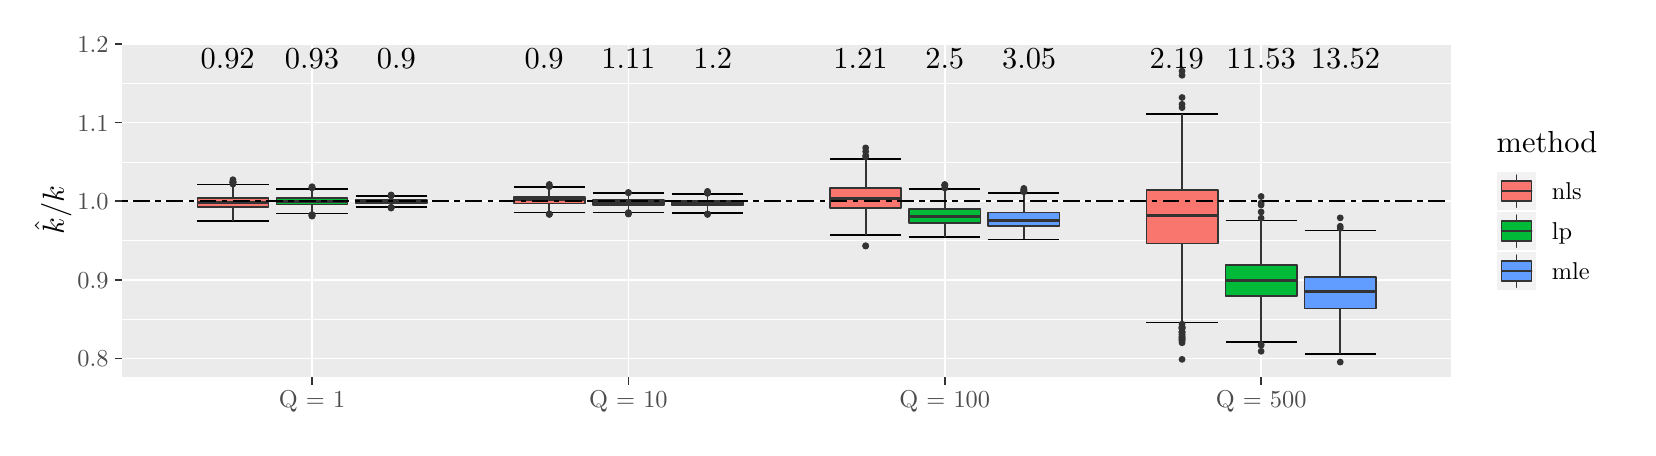
\begin{tikzpicture}[x=1pt,y=1pt]
\definecolor{fillColor}{RGB}{255,255,255}
\path[use as bounding box,fill=fillColor,fill opacity=0.00] (0,0) rectangle (578.16,144.54);
\begin{scope}
\path[clip] (  0.00,  0.00) rectangle (578.16,144.54);
\definecolor{drawColor}{RGB}{255,255,255}
\definecolor{fillColor}{RGB}{255,255,255}

\path[draw=drawColor,line width= 0.6pt,line join=round,line cap=round,fill=fillColor] (  0.00,  0.00) rectangle (578.16,144.54);
\end{scope}
\begin{scope}
\path[clip] ( 34.16, 18.22) rectangle (514.31,139.04);
\definecolor{fillColor}{gray}{0.92}

\path[fill=fillColor] ( 34.16, 18.22) rectangle (514.31,139.04);
\definecolor{drawColor}{RGB}{255,255,255}

\path[draw=drawColor,line width= 0.3pt,line join=round] ( 34.16, 39.18) --
	(514.31, 39.18);

\path[draw=drawColor,line width= 0.3pt,line join=round] ( 34.16, 67.60) --
	(514.31, 67.60);

\path[draw=drawColor,line width= 0.3pt,line join=round] ( 34.16, 96.01) --
	(514.31, 96.01);

\path[draw=drawColor,line width= 0.3pt,line join=round] ( 34.16,124.42) --
	(514.31,124.42);

\path[draw=drawColor,line width= 0.6pt,line join=round] ( 34.16, 24.98) --
	(514.31, 24.98);

\path[draw=drawColor,line width= 0.6pt,line join=round] ( 34.16, 53.39) --
	(514.31, 53.39);

\path[draw=drawColor,line width= 0.6pt,line join=round] ( 34.16, 81.80) --
	(514.31, 81.80);

\path[draw=drawColor,line width= 0.6pt,line join=round] ( 34.16,110.22) --
	(514.31,110.22);

\path[draw=drawColor,line width= 0.6pt,line join=round] ( 34.16,138.63) --
	(514.31,138.63);

\path[draw=drawColor,line width= 0.6pt,line join=round] (102.75, 18.22) --
	(102.75,139.04);

\path[draw=drawColor,line width= 0.6pt,line join=round] (217.07, 18.22) --
	(217.07,139.04);

\path[draw=drawColor,line width= 0.6pt,line join=round] (331.39, 18.22) --
	(331.39,139.04);

\path[draw=drawColor,line width= 0.6pt,line join=round] (445.71, 18.22) --
	(445.71,139.04);
\definecolor{drawColor}{RGB}{0,0,0}

\path[draw=drawColor,line width= 0.6pt,line join=round] ( 61.31, 87.90) --
	( 87.03, 87.90);

\path[draw=drawColor,line width= 0.6pt,line join=round] ( 74.17, 87.90) --
	( 74.17, 74.79);

\path[draw=drawColor,line width= 0.6pt,line join=round] ( 61.31, 74.79) --
	( 87.03, 74.79);

\path[draw=drawColor,line width= 0.6pt,line join=round] ( 89.89, 86.33) --
	(115.61, 86.33);

\path[draw=drawColor,line width= 0.6pt,line join=round] (102.75, 86.33) --
	(102.75, 77.39);

\path[draw=drawColor,line width= 0.6pt,line join=round] ( 89.89, 77.39) --
	(115.61, 77.39);

\path[draw=drawColor,line width= 0.6pt,line join=round] (118.47, 83.67) --
	(144.19, 83.67);

\path[draw=drawColor,line width= 0.6pt,line join=round] (131.33, 83.67) --
	(131.33, 79.68);

\path[draw=drawColor,line width= 0.6pt,line join=round] (118.47, 79.68) --
	(144.19, 79.68);

\path[draw=drawColor,line width= 0.6pt,line join=round] (175.63, 87.02) --
	(201.35, 87.02);

\path[draw=drawColor,line width= 0.6pt,line join=round] (188.49, 87.02) --
	(188.49, 77.72);

\path[draw=drawColor,line width= 0.6pt,line join=round] (175.63, 77.72) --
	(201.35, 77.72);

\path[draw=drawColor,line width= 0.6pt,line join=round] (204.21, 84.72) --
	(229.93, 84.72);

\path[draw=drawColor,line width= 0.6pt,line join=round] (217.07, 84.72) --
	(217.07, 77.79);

\path[draw=drawColor,line width= 0.6pt,line join=round] (204.21, 77.79) --
	(229.93, 77.79);

\path[draw=drawColor,line width= 0.6pt,line join=round] (232.79, 84.46) --
	(258.51, 84.46);

\path[draw=drawColor,line width= 0.6pt,line join=round] (245.65, 84.46) --
	(245.65, 77.64);

\path[draw=drawColor,line width= 0.6pt,line join=round] (232.79, 77.64) --
	(258.51, 77.64);

\path[draw=drawColor,line width= 0.6pt,line join=round] (289.95, 97.11) --
	(315.67, 97.11);

\path[draw=drawColor,line width= 0.6pt,line join=round] (302.81, 97.11) --
	(302.81, 69.55);

\path[draw=drawColor,line width= 0.6pt,line join=round] (289.95, 69.55) --
	(315.67, 69.55);

\path[draw=drawColor,line width= 0.6pt,line join=round] (318.53, 86.15) --
	(344.25, 86.15);

\path[draw=drawColor,line width= 0.6pt,line join=round] (331.39, 86.15) --
	(331.39, 68.79);

\path[draw=drawColor,line width= 0.6pt,line join=round] (318.53, 68.79) --
	(344.25, 68.79);

\path[draw=drawColor,line width= 0.6pt,line join=round] (347.11, 84.72) --
	(372.83, 84.72);

\path[draw=drawColor,line width= 0.6pt,line join=round] (359.97, 84.72) --
	(359.97, 68.02);

\path[draw=drawColor,line width= 0.6pt,line join=round] (347.11, 68.02) --
	(372.83, 68.02);

\path[draw=drawColor,line width= 0.6pt,line join=round] (404.27,113.28) --
	(430.00,113.28);

\path[draw=drawColor,line width= 0.6pt,line join=round] (417.13,113.28) --
	(417.13, 38.06);

\path[draw=drawColor,line width= 0.6pt,line join=round] (404.27, 38.06) --
	(430.00, 38.06);

\path[draw=drawColor,line width= 0.6pt,line join=round] (432.85, 74.82) --
	(458.58, 74.82);

\path[draw=drawColor,line width= 0.6pt,line join=round] (445.71, 74.82) --
	(445.71, 30.94);

\path[draw=drawColor,line width= 0.6pt,line join=round] (432.85, 30.94) --
	(458.58, 30.94);

\path[draw=drawColor,line width= 0.6pt,line join=round] (461.43, 71.20) --
	(487.16, 71.20);

\path[draw=drawColor,line width= 0.6pt,line join=round] (474.29, 71.20) --
	(474.29, 26.65);

\path[draw=drawColor,line width= 0.6pt,line join=round] (461.43, 26.65) --
	(487.16, 26.65);
\definecolor{drawColor}{gray}{0.20}
\definecolor{fillColor}{gray}{0.20}

\path[draw=drawColor,line width= 0.4pt,line join=round,line cap=round,fill=fillColor] ( 74.17, 88.78) circle (  1.02);

\path[draw=drawColor,line width= 0.4pt,line join=round,line cap=round,fill=fillColor] ( 74.17, 88.79) circle (  1.02);

\path[draw=drawColor,line width= 0.4pt,line join=round,line cap=round,fill=fillColor] ( 74.17, 88.02) circle (  1.02);

\path[draw=drawColor,line width= 0.4pt,line join=round,line cap=round,fill=fillColor] ( 74.17, 88.52) circle (  1.02);

\path[draw=drawColor,line width= 0.4pt,line join=round,line cap=round,fill=fillColor] ( 74.17, 89.60) circle (  1.02);

\path[draw=drawColor,line width= 0.4pt,line join=round,line cap=round,fill=fillColor] ( 74.17, 88.91) circle (  1.02);

\path[draw=drawColor,line width= 0.4pt,line join=round,line cap=round,fill=fillColor] ( 74.17, 88.61) circle (  1.02);

\path[draw=drawColor,line width= 0.6pt,line join=round] ( 74.17, 83.00) -- ( 74.17, 87.90);

\path[draw=drawColor,line width= 0.6pt,line join=round] ( 74.17, 79.67) -- ( 74.17, 74.79);
\definecolor{fillColor}{RGB}{248,118,109}

\path[draw=drawColor,line width= 0.6pt,line join=round,line cap=round,fill=fillColor] ( 61.31, 83.00) --
	( 61.31, 79.67) --
	( 87.03, 79.67) --
	( 87.03, 83.00) --
	( 61.31, 83.00) --
	cycle;

\path[draw=drawColor,line width= 1.1pt,line join=round] ( 61.31, 81.28) -- ( 87.03, 81.28);
\definecolor{fillColor}{gray}{0.20}

\path[draw=drawColor,line width= 0.4pt,line join=round,line cap=round,fill=fillColor] (102.75, 76.59) circle (  1.02);

\path[draw=drawColor,line width= 0.4pt,line join=round,line cap=round,fill=fillColor] (102.75, 77.00) circle (  1.02);

\path[draw=drawColor,line width= 0.4pt,line join=round,line cap=round,fill=fillColor] (102.75, 76.83) circle (  1.02);

\path[draw=drawColor,line width= 0.4pt,line join=round,line cap=round,fill=fillColor] (102.75, 86.85) circle (  1.02);

\path[draw=drawColor,line width= 0.4pt,line join=round,line cap=round,fill=fillColor] (102.75, 76.56) circle (  1.02);

\path[draw=drawColor,line width= 0.4pt,line join=round,line cap=round,fill=fillColor] (102.75, 87.07) circle (  1.02);

\path[draw=drawColor,line width= 0.4pt,line join=round,line cap=round,fill=fillColor] (102.75, 76.45) circle (  1.02);

\path[draw=drawColor,line width= 0.4pt,line join=round,line cap=round,fill=fillColor] (102.75, 86.64) circle (  1.02);

\path[draw=drawColor,line width= 0.6pt,line join=round] (102.75, 82.98) -- (102.75, 86.33);

\path[draw=drawColor,line width= 0.6pt,line join=round] (102.75, 80.65) -- (102.75, 77.39);
\definecolor{fillColor}{RGB}{0,186,56}

\path[draw=drawColor,line width= 0.6pt,line join=round,line cap=round,fill=fillColor] ( 89.89, 82.98) --
	( 89.89, 80.65) --
	(115.61, 80.65) --
	(115.61, 82.98) --
	( 89.89, 82.98) --
	cycle;

\path[draw=drawColor,line width= 1.1pt,line join=round] ( 89.89, 81.70) -- (115.61, 81.70);
\definecolor{fillColor}{gray}{0.20}

\path[draw=drawColor,line width= 0.4pt,line join=round,line cap=round,fill=fillColor] (131.33, 84.04) circle (  1.02);

\path[draw=drawColor,line width= 0.4pt,line join=round,line cap=round,fill=fillColor] (131.33, 79.60) circle (  1.02);

\path[draw=drawColor,line width= 0.4pt,line join=round,line cap=round,fill=fillColor] (131.33, 83.76) circle (  1.02);

\path[draw=drawColor,line width= 0.4pt,line join=round,line cap=round,fill=fillColor] (131.33, 84.05) circle (  1.02);

\path[draw=drawColor,line width= 0.4pt,line join=round,line cap=round,fill=fillColor] (131.33, 79.50) circle (  1.02);

\path[draw=drawColor,line width= 0.4pt,line join=round,line cap=round,fill=fillColor] (131.33, 79.34) circle (  1.02);

\path[draw=drawColor,line width= 0.4pt,line join=round,line cap=round,fill=fillColor] (131.33, 83.84) circle (  1.02);

\path[draw=drawColor,line width= 0.4pt,line join=round,line cap=round,fill=fillColor] (131.33, 79.58) circle (  1.02);

\path[draw=drawColor,line width= 0.6pt,line join=round] (131.33, 82.18) -- (131.33, 83.67);

\path[draw=drawColor,line width= 0.6pt,line join=round] (131.33, 81.18) -- (131.33, 79.68);
\definecolor{fillColor}{RGB}{97,156,255}

\path[draw=drawColor,line width= 0.6pt,line join=round,line cap=round,fill=fillColor] (118.47, 82.18) --
	(118.47, 81.18) --
	(144.19, 81.18) --
	(144.19, 82.18) --
	(118.47, 82.18) --
	cycle;

\path[draw=drawColor,line width= 1.1pt,line join=round] (118.47, 81.70) -- (144.19, 81.70);
\definecolor{fillColor}{gray}{0.20}

\path[draw=drawColor,line width= 0.4pt,line join=round,line cap=round,fill=fillColor] (188.49, 77.20) circle (  1.02);

\path[draw=drawColor,line width= 0.4pt,line join=round,line cap=round,fill=fillColor] (188.49, 87.35) circle (  1.02);

\path[draw=drawColor,line width= 0.4pt,line join=round,line cap=round,fill=fillColor] (188.49, 87.18) circle (  1.02);

\path[draw=drawColor,line width= 0.4pt,line join=round,line cap=round,fill=fillColor] (188.49, 87.13) circle (  1.02);

\path[draw=drawColor,line width= 0.4pt,line join=round,line cap=round,fill=fillColor] (188.49, 77.13) circle (  1.02);

\path[draw=drawColor,line width= 0.4pt,line join=round,line cap=round,fill=fillColor] (188.49, 87.88) circle (  1.02);

\path[draw=drawColor,line width= 0.4pt,line join=round,line cap=round,fill=fillColor] (188.49, 77.07) circle (  1.02);

\path[draw=drawColor,line width= 0.6pt,line join=round] (188.49, 83.40) -- (188.49, 87.02);

\path[draw=drawColor,line width= 0.6pt,line join=round] (188.49, 80.97) -- (188.49, 77.72);
\definecolor{fillColor}{RGB}{248,118,109}

\path[draw=drawColor,line width= 0.6pt,line join=round,line cap=round,fill=fillColor] (175.63, 83.40) --
	(175.63, 80.97) --
	(201.35, 80.97) --
	(201.35, 83.40) --
	(175.63, 83.40) --
	cycle;

\path[draw=drawColor,line width= 1.1pt,line join=round] (175.63, 82.30) -- (201.35, 82.30);
\definecolor{fillColor}{gray}{0.20}

\path[draw=drawColor,line width= 0.4pt,line join=round,line cap=round,fill=fillColor] (217.07, 84.99) circle (  1.02);

\path[draw=drawColor,line width= 0.4pt,line join=round,line cap=round,fill=fillColor] (217.07, 77.18) circle (  1.02);

\path[draw=drawColor,line width= 0.4pt,line join=round,line cap=round,fill=fillColor] (217.07, 77.34) circle (  1.02);

\path[draw=drawColor,line width= 0.4pt,line join=round,line cap=round,fill=fillColor] (217.07, 77.63) circle (  1.02);

\path[draw=drawColor,line width= 0.4pt,line join=round,line cap=round,fill=fillColor] (217.07, 77.69) circle (  1.02);

\path[draw=drawColor,line width= 0.4pt,line join=round,line cap=round,fill=fillColor] (217.07, 84.86) circle (  1.02);

\path[draw=drawColor,line width= 0.6pt,line join=round] (217.07, 82.18) -- (217.07, 84.72);

\path[draw=drawColor,line width= 0.6pt,line join=round] (217.07, 80.41) -- (217.07, 77.79);
\definecolor{fillColor}{RGB}{0,186,56}

\path[draw=drawColor,line width= 0.6pt,line join=round,line cap=round,fill=fillColor] (204.21, 82.18) --
	(204.21, 80.41) --
	(229.93, 80.41) --
	(229.93, 82.18) --
	(204.21, 82.18) --
	cycle;

\path[draw=drawColor,line width= 1.1pt,line join=round] (204.21, 81.33) -- (229.93, 81.33);
\definecolor{fillColor}{gray}{0.20}

\path[draw=drawColor,line width= 0.4pt,line join=round,line cap=round,fill=fillColor] (245.65, 85.38) circle (  1.02);

\path[draw=drawColor,line width= 0.4pt,line join=round,line cap=round,fill=fillColor] (245.65, 77.05) circle (  1.02);

\path[draw=drawColor,line width= 0.4pt,line join=round,line cap=round,fill=fillColor] (245.65, 77.23) circle (  1.02);

\path[draw=drawColor,line width= 0.4pt,line join=round,line cap=round,fill=fillColor] (245.65, 84.68) circle (  1.02);

\path[draw=drawColor,line width= 0.4pt,line join=round,line cap=round,fill=fillColor] (245.65, 84.76) circle (  1.02);

\path[draw=drawColor,line width= 0.6pt,line join=round] (245.65, 82.01) -- (245.65, 84.46);

\path[draw=drawColor,line width= 0.6pt,line join=round] (245.65, 80.23) -- (245.65, 77.64);
\definecolor{fillColor}{RGB}{97,156,255}

\path[draw=drawColor,line width= 0.6pt,line join=round,line cap=round,fill=fillColor] (232.79, 82.01) --
	(232.79, 80.23) --
	(258.51, 80.23) --
	(258.51, 82.01) --
	(232.79, 82.01) --
	cycle;

\path[draw=drawColor,line width= 1.1pt,line join=round] (232.79, 81.09) -- (258.51, 81.09);
\definecolor{fillColor}{gray}{0.20}

\path[draw=drawColor,line width= 0.4pt,line join=round,line cap=round,fill=fillColor] (302.81,101.11) circle (  1.02);

\path[draw=drawColor,line width= 0.4pt,line join=round,line cap=round,fill=fillColor] (302.81, 97.85) circle (  1.02);

\path[draw=drawColor,line width= 0.4pt,line join=round,line cap=round,fill=fillColor] (302.81, 99.77) circle (  1.02);

\path[draw=drawColor,line width= 0.4pt,line join=round,line cap=round,fill=fillColor] (302.81, 65.64) circle (  1.02);

\path[draw=drawColor,line width= 0.4pt,line join=round,line cap=round,fill=fillColor] (302.81, 98.32) circle (  1.02);

\path[draw=drawColor,line width= 0.4pt,line join=round,line cap=round,fill=fillColor] (302.81, 65.73) circle (  1.02);

\path[draw=drawColor,line width= 0.6pt,line join=round] (302.81, 86.49) -- (302.81, 97.11);

\path[draw=drawColor,line width= 0.6pt,line join=round] (302.81, 79.35) -- (302.81, 69.55);
\definecolor{fillColor}{RGB}{248,118,109}

\path[draw=drawColor,line width= 0.6pt,line join=round,line cap=round,fill=fillColor] (289.95, 86.49) --
	(289.95, 79.35) --
	(315.67, 79.35) --
	(315.67, 86.49) --
	(289.95, 86.49) --
	cycle;

\path[draw=drawColor,line width= 1.1pt,line join=round] (289.95, 82.84) -- (315.67, 82.84);
\definecolor{fillColor}{gray}{0.20}

\path[draw=drawColor,line width= 0.4pt,line join=round,line cap=round,fill=fillColor] (331.39, 87.54) circle (  1.02);

\path[draw=drawColor,line width= 0.4pt,line join=round,line cap=round,fill=fillColor] (331.39, 87.87) circle (  1.02);

\path[draw=drawColor,line width= 0.4pt,line join=round,line cap=round,fill=fillColor] (331.39, 87.57) circle (  1.02);

\path[draw=drawColor,line width= 0.4pt,line join=round,line cap=round,fill=fillColor] (331.39, 86.59) circle (  1.02);

\path[draw=drawColor,line width= 0.6pt,line join=round] (331.39, 78.95) -- (331.39, 86.15);

\path[draw=drawColor,line width= 0.6pt,line join=round] (331.39, 73.93) -- (331.39, 68.79);
\definecolor{fillColor}{RGB}{0,186,56}

\path[draw=drawColor,line width= 0.6pt,line join=round,line cap=round,fill=fillColor] (318.53, 78.95) --
	(318.53, 73.93) --
	(344.25, 73.93) --
	(344.25, 78.95) --
	(318.53, 78.95) --
	cycle;

\path[draw=drawColor,line width= 1.1pt,line join=round] (318.53, 76.38) -- (344.25, 76.38);
\definecolor{fillColor}{gray}{0.20}

\path[draw=drawColor,line width= 0.4pt,line join=round,line cap=round,fill=fillColor] (359.97, 86.00) circle (  1.02);

\path[draw=drawColor,line width= 0.4pt,line join=round,line cap=round,fill=fillColor] (359.97, 85.52) circle (  1.02);

\path[draw=drawColor,line width= 0.4pt,line join=round,line cap=round,fill=fillColor] (359.97, 85.38) circle (  1.02);

\path[draw=drawColor,line width= 0.4pt,line join=round,line cap=round,fill=fillColor] (359.97, 85.93) circle (  1.02);

\path[draw=drawColor,line width= 0.4pt,line join=round,line cap=round,fill=fillColor] (359.97, 85.41) circle (  1.02);

\path[draw=drawColor,line width= 0.4pt,line join=round,line cap=round,fill=fillColor] (359.97, 85.24) circle (  1.02);

\path[draw=drawColor,line width= 0.4pt,line join=round,line cap=round,fill=fillColor] (359.97, 86.46) circle (  1.02);

\path[draw=drawColor,line width= 0.4pt,line join=round,line cap=round,fill=fillColor] (359.97, 85.72) circle (  1.02);

\path[draw=drawColor,line width= 0.6pt,line join=round] (359.97, 77.77) -- (359.97, 84.72);

\path[draw=drawColor,line width= 0.6pt,line join=round] (359.97, 72.87) -- (359.97, 68.02);
\definecolor{fillColor}{RGB}{97,156,255}

\path[draw=drawColor,line width= 0.6pt,line join=round,line cap=round,fill=fillColor] (347.11, 77.77) --
	(347.11, 72.87) --
	(372.83, 72.87) --
	(372.83, 77.77) --
	(347.11, 77.77) --
	cycle;

\path[draw=drawColor,line width= 1.1pt,line join=round] (347.11, 74.94) -- (372.83, 74.94);
\definecolor{fillColor}{gray}{0.20}

\path[draw=drawColor,line width= 0.4pt,line join=round,line cap=round,fill=fillColor] (417.13,115.65) circle (  1.02);

\path[draw=drawColor,line width= 0.4pt,line join=round,line cap=round,fill=fillColor] (417.13, 32.83) circle (  1.02);

\path[draw=drawColor,line width= 0.4pt,line join=round,line cap=round,fill=fillColor] (417.13, 34.58) circle (  1.02);

\path[draw=drawColor,line width= 0.4pt,line join=round,line cap=round,fill=fillColor] (417.13, 33.59) circle (  1.02);

\path[draw=drawColor,line width= 0.4pt,line join=round,line cap=round,fill=fillColor] (417.13,128.84) circle (  1.02);

\path[draw=drawColor,line width= 0.4pt,line join=round,line cap=round,fill=fillColor] (417.13,119.31) circle (  1.02);

\path[draw=drawColor,line width= 0.4pt,line join=round,line cap=round,fill=fillColor] (417.13, 31.56) circle (  1.02);

\path[draw=drawColor,line width= 0.4pt,line join=round,line cap=round,fill=fillColor] (417.13, 33.64) circle (  1.02);

\path[draw=drawColor,line width= 0.4pt,line join=round,line cap=round,fill=fillColor] (417.13, 32.75) circle (  1.02);

\path[draw=drawColor,line width= 0.4pt,line join=round,line cap=round,fill=fillColor] (417.13, 30.68) circle (  1.02);

\path[draw=drawColor,line width= 0.4pt,line join=round,line cap=round,fill=fillColor] (417.13,127.33) circle (  1.02);

\path[draw=drawColor,line width= 0.4pt,line join=round,line cap=round,fill=fillColor] (417.13, 34.67) circle (  1.02);

\path[draw=drawColor,line width= 0.4pt,line join=round,line cap=round,fill=fillColor] (417.13, 24.68) circle (  1.02);

\path[draw=drawColor,line width= 0.4pt,line join=round,line cap=round,fill=fillColor] (417.13, 36.50) circle (  1.02);

\path[draw=drawColor,line width= 0.4pt,line join=round,line cap=round,fill=fillColor] (417.13, 36.25) circle (  1.02);

\path[draw=drawColor,line width= 0.4pt,line join=round,line cap=round,fill=fillColor] (417.13, 34.35) circle (  1.02);

\path[draw=drawColor,line width= 0.4pt,line join=round,line cap=round,fill=fillColor] (417.13,116.86) circle (  1.02);

\path[draw=drawColor,line width= 0.4pt,line join=round,line cap=round,fill=fillColor] (417.13, 32.03) circle (  1.02);

\path[draw=drawColor,line width= 0.4pt,line join=round,line cap=round,fill=fillColor] (417.13, 36.11) circle (  1.02);

\path[draw=drawColor,line width= 0.4pt,line join=round,line cap=round,fill=fillColor] (417.13, 31.35) circle (  1.02);

\path[draw=drawColor,line width= 0.4pt,line join=round,line cap=round,fill=fillColor] (417.13, 32.03) circle (  1.02);

\path[draw=drawColor,line width= 0.4pt,line join=round,line cap=round,fill=fillColor] (417.13, 35.70) circle (  1.02);

\path[draw=drawColor,line width= 0.4pt,line join=round,line cap=round,fill=fillColor] (417.13, 32.52) circle (  1.02);

\path[draw=drawColor,line width= 0.4pt,line join=round,line cap=round,fill=fillColor] (417.13, 37.40) circle (  1.02);

\path[draw=drawColor,line width= 0.4pt,line join=round,line cap=round,fill=fillColor] (417.13, 35.92) circle (  1.02);

\path[draw=drawColor,line width= 0.6pt,line join=round] (417.13, 86.00) -- (417.13,113.28);

\path[draw=drawColor,line width= 0.6pt,line join=round] (417.13, 66.58) -- (417.13, 38.06);
\definecolor{fillColor}{RGB}{248,118,109}

\path[draw=drawColor,line width= 0.6pt,line join=round,line cap=round,fill=fillColor] (404.27, 86.00) --
	(404.27, 66.58) --
	(430.00, 66.58) --
	(430.00, 86.00) --
	(404.27, 86.00) --
	cycle;

\path[draw=drawColor,line width= 1.1pt,line join=round] (404.27, 76.66) -- (430.00, 76.66);
\definecolor{fillColor}{gray}{0.20}

\path[draw=drawColor,line width= 0.4pt,line join=round,line cap=round,fill=fillColor] (445.71, 81.20) circle (  1.02);

\path[draw=drawColor,line width= 0.4pt,line join=round,line cap=round,fill=fillColor] (445.71, 75.69) circle (  1.02);

\path[draw=drawColor,line width= 0.4pt,line join=round,line cap=round,fill=fillColor] (445.71, 83.54) circle (  1.02);

\path[draw=drawColor,line width= 0.4pt,line join=round,line cap=round,fill=fillColor] (445.71, 77.95) circle (  1.02);

\path[draw=drawColor,line width= 0.4pt,line join=round,line cap=round,fill=fillColor] (445.71, 27.61) circle (  1.02);

\path[draw=drawColor,line width= 0.4pt,line join=round,line cap=round,fill=fillColor] (445.71, 29.79) circle (  1.02);

\path[draw=drawColor,line width= 0.4pt,line join=round,line cap=round,fill=fillColor] (445.71, 30.06) circle (  1.02);

\path[draw=drawColor,line width= 0.4pt,line join=round,line cap=round,fill=fillColor] (445.71, 80.46) circle (  1.02);

\path[draw=drawColor,line width= 0.6pt,line join=round] (445.71, 58.84) -- (445.71, 74.82);

\path[draw=drawColor,line width= 0.6pt,line join=round] (445.71, 47.64) -- (445.71, 30.94);
\definecolor{fillColor}{RGB}{0,186,56}

\path[draw=drawColor,line width= 0.6pt,line join=round,line cap=round,fill=fillColor] (432.85, 58.84) --
	(432.85, 47.64) --
	(458.58, 47.64) --
	(458.58, 58.84) --
	(432.85, 58.84) --
	cycle;

\path[draw=drawColor,line width= 1.1pt,line join=round] (432.85, 53.11) -- (458.58, 53.11);
\definecolor{fillColor}{gray}{0.20}

\path[draw=drawColor,line width= 0.4pt,line join=round,line cap=round,fill=fillColor] (474.29, 23.71) circle (  1.02);

\path[draw=drawColor,line width= 0.4pt,line join=round,line cap=round,fill=fillColor] (474.29, 75.82) circle (  1.02);

\path[draw=drawColor,line width= 0.4pt,line join=round,line cap=round,fill=fillColor] (474.29, 72.06) circle (  1.02);

\path[draw=drawColor,line width= 0.4pt,line join=round,line cap=round,fill=fillColor] (474.29, 72.78) circle (  1.02);

\path[draw=drawColor,line width= 0.6pt,line join=round] (474.29, 54.47) -- (474.29, 71.20);

\path[draw=drawColor,line width= 0.6pt,line join=round] (474.29, 43.10) -- (474.29, 26.65);
\definecolor{fillColor}{RGB}{97,156,255}

\path[draw=drawColor,line width= 0.6pt,line join=round,line cap=round,fill=fillColor] (461.43, 54.47) --
	(461.43, 43.10) --
	(487.16, 43.10) --
	(487.16, 54.47) --
	(461.43, 54.47) --
	cycle;

\path[draw=drawColor,line width= 1.1pt,line join=round] (461.43, 49.11) -- (487.16, 49.11);
\definecolor{drawColor}{RGB}{0,0,0}

\path[draw=drawColor,line width= 0.6pt,dash pattern=on 2pt off 2pt on 6pt off 2pt ,line join=round] ( 34.16, 81.80) -- (514.31, 81.80);

\node[text=drawColor,anchor=base,inner sep=0pt, outer sep=0pt, scale=  1.10] at (133.23,129.75) {0.9};

\node[text=drawColor,anchor=base,inner sep=0pt, outer sep=0pt, scale=  1.10] at (102.75,129.75) {0.93};

\node[text=drawColor,anchor=base,inner sep=0pt, outer sep=0pt, scale=  1.10] at ( 72.26,129.75) {0.92};

\node[text=drawColor,anchor=base,inner sep=0pt, outer sep=0pt, scale=  1.10] at (247.56,129.75) {1.2};

\node[text=drawColor,anchor=base,inner sep=0pt, outer sep=0pt, scale=  1.10] at (217.07,129.75) {1.11};

\node[text=drawColor,anchor=base,inner sep=0pt, outer sep=0pt, scale=  1.10] at (186.59,129.75) {0.9};

\node[text=drawColor,anchor=base,inner sep=0pt, outer sep=0pt, scale=  1.10] at (361.88,129.75) {3.05};

\node[text=drawColor,anchor=base,inner sep=0pt, outer sep=0pt, scale=  1.10] at (331.39,129.75) {2.5};

\node[text=drawColor,anchor=base,inner sep=0pt, outer sep=0pt, scale=  1.10] at (300.91,129.75) {1.21};

\node[text=drawColor,anchor=base,inner sep=0pt, outer sep=0pt, scale=  1.10] at (476.20,129.75) {13.52};

\node[text=drawColor,anchor=base,inner sep=0pt, outer sep=0pt, scale=  1.10] at (445.71,129.75) {11.53};

\node[text=drawColor,anchor=base,inner sep=0pt, outer sep=0pt, scale=  1.10] at (415.23,129.75) {2.19};
\end{scope}
\begin{scope}
\path[clip] (  0.00,  0.00) rectangle (578.16,144.54);
\definecolor{drawColor}{gray}{0.30}

\node[text=drawColor,anchor=base east,inner sep=0pt, outer sep=0pt, scale=  0.88] at ( 29.21, 21.95) {0.8};

\node[text=drawColor,anchor=base east,inner sep=0pt, outer sep=0pt, scale=  0.88] at ( 29.21, 50.36) {0.9};

\node[text=drawColor,anchor=base east,inner sep=0pt, outer sep=0pt, scale=  0.88] at ( 29.21, 78.77) {1.0};

\node[text=drawColor,anchor=base east,inner sep=0pt, outer sep=0pt, scale=  0.88] at ( 29.21,107.19) {1.1};

\node[text=drawColor,anchor=base east,inner sep=0pt, outer sep=0pt, scale=  0.88] at ( 29.21,135.60) {1.2};
\end{scope}
\begin{scope}
\path[clip] (  0.00,  0.00) rectangle (578.16,144.54);
\definecolor{drawColor}{gray}{0.20}

\path[draw=drawColor,line width= 0.6pt,line join=round] ( 31.41, 24.98) --
	( 34.16, 24.98);

\path[draw=drawColor,line width= 0.6pt,line join=round] ( 31.41, 53.39) --
	( 34.16, 53.39);

\path[draw=drawColor,line width= 0.6pt,line join=round] ( 31.41, 81.80) --
	( 34.16, 81.80);

\path[draw=drawColor,line width= 0.6pt,line join=round] ( 31.41,110.22) --
	( 34.16,110.22);

\path[draw=drawColor,line width= 0.6pt,line join=round] ( 31.41,138.63) --
	( 34.16,138.63);
\end{scope}
\begin{scope}
\path[clip] (  0.00,  0.00) rectangle (578.16,144.54);
\definecolor{drawColor}{gray}{0.20}

\path[draw=drawColor,line width= 0.6pt,line join=round] (102.75, 15.47) --
	(102.75, 18.22);

\path[draw=drawColor,line width= 0.6pt,line join=round] (217.07, 15.47) --
	(217.07, 18.22);

\path[draw=drawColor,line width= 0.6pt,line join=round] (331.39, 15.47) --
	(331.39, 18.22);

\path[draw=drawColor,line width= 0.6pt,line join=round] (445.71, 15.47) --
	(445.71, 18.22);
\end{scope}
\begin{scope}
\path[clip] (  0.00,  0.00) rectangle (578.16,144.54);
\definecolor{drawColor}{gray}{0.30}

\node[text=drawColor,anchor=base,inner sep=0pt, outer sep=0pt, scale=  0.88] at (102.75,  7.21) {Q = 1};

\node[text=drawColor,anchor=base,inner sep=0pt, outer sep=0pt, scale=  0.88] at (217.07,  7.21) {Q = 10};

\node[text=drawColor,anchor=base,inner sep=0pt, outer sep=0pt, scale=  0.88] at (331.39,  7.21) {Q = 100};

\node[text=drawColor,anchor=base,inner sep=0pt, outer sep=0pt, scale=  0.88] at (445.71,  7.21) {Q = 500};
\end{scope}
\begin{scope}
\path[clip] (  0.00,  0.00) rectangle (578.16,144.54);
\definecolor{drawColor}{RGB}{0,0,0}

\node[text=drawColor,rotate= 90.00,anchor=base,inner sep=0pt, outer sep=0pt, scale=  1.10] at ( 13.08, 78.63) {$\hat{k}/k$};
\end{scope}
\begin{scope}
\path[clip] (  0.00,  0.00) rectangle (578.16,144.54);
\definecolor{fillColor}{RGB}{255,255,255}

\path[fill=fillColor] (525.31, 43.84) rectangle (572.66,113.42);
\end{scope}
\begin{scope}
\path[clip] (  0.00,  0.00) rectangle (578.16,144.54);
\definecolor{drawColor}{RGB}{0,0,0}

\node[text=drawColor,anchor=base west,inner sep=0pt, outer sep=0pt, scale=  1.10] at (530.81, 99.27) {method};
\end{scope}
\begin{scope}
\path[clip] (  0.00,  0.00) rectangle (578.16,144.54);
\definecolor{drawColor}{RGB}{255,255,255}
\definecolor{fillColor}{gray}{0.95}

\path[draw=drawColor,line width= 0.6pt,line join=round,line cap=round,fill=fillColor] (530.81, 78.25) rectangle (545.26, 92.70);
\end{scope}
\begin{scope}
\path[clip] (  0.00,  0.00) rectangle (578.16,144.54);
\definecolor{drawColor}{gray}{0.20}

\path[draw=drawColor,line width= 0.6pt,line join=round,line cap=round] (538.03, 79.70) --
	(538.03, 81.86);

\path[draw=drawColor,line width= 0.6pt,line join=round,line cap=round] (538.03, 89.09) --
	(538.03, 91.26);
\definecolor{fillColor}{RGB}{248,118,109}

\path[draw=drawColor,line width= 0.6pt,line join=round,line cap=round,fill=fillColor] (532.61, 81.86) rectangle (543.45, 89.09);

\path[draw=drawColor,line width= 0.6pt,line join=round,line cap=round] (532.61, 85.48) --
	(543.45, 85.48);
\end{scope}
\begin{scope}
\path[clip] (  0.00,  0.00) rectangle (578.16,144.54);
\definecolor{drawColor}{RGB}{255,255,255}
\definecolor{fillColor}{gray}{0.95}

\path[draw=drawColor,line width= 0.6pt,line join=round,line cap=round,fill=fillColor] (530.81, 63.80) rectangle (545.26, 78.25);
\end{scope}
\begin{scope}
\path[clip] (  0.00,  0.00) rectangle (578.16,144.54);
\definecolor{drawColor}{gray}{0.20}

\path[draw=drawColor,line width= 0.6pt,line join=round,line cap=round] (538.03, 65.24) --
	(538.03, 67.41);

\path[draw=drawColor,line width= 0.6pt,line join=round,line cap=round] (538.03, 74.64) --
	(538.03, 76.81);
\definecolor{fillColor}{RGB}{0,186,56}

\path[draw=drawColor,line width= 0.6pt,line join=round,line cap=round,fill=fillColor] (532.61, 67.41) rectangle (543.45, 74.64);

\path[draw=drawColor,line width= 0.6pt,line join=round,line cap=round] (532.61, 71.02) --
	(543.45, 71.02);
\end{scope}
\begin{scope}
\path[clip] (  0.00,  0.00) rectangle (578.16,144.54);
\definecolor{drawColor}{RGB}{255,255,255}
\definecolor{fillColor}{gray}{0.95}

\path[draw=drawColor,line width= 0.6pt,line join=round,line cap=round,fill=fillColor] (530.81, 49.34) rectangle (545.26, 63.80);
\end{scope}
\begin{scope}
\path[clip] (  0.00,  0.00) rectangle (578.16,144.54);
\definecolor{drawColor}{gray}{0.20}

\path[draw=drawColor,line width= 0.6pt,line join=round,line cap=round] (538.03, 50.79) --
	(538.03, 52.96);

\path[draw=drawColor,line width= 0.6pt,line join=round,line cap=round] (538.03, 60.18) --
	(538.03, 62.35);
\definecolor{fillColor}{RGB}{97,156,255}

\path[draw=drawColor,line width= 0.6pt,line join=round,line cap=round,fill=fillColor] (532.61, 52.96) rectangle (543.45, 60.18);

\path[draw=drawColor,line width= 0.6pt,line join=round,line cap=round] (532.61, 56.57) --
	(543.45, 56.57);
\end{scope}
\begin{scope}
\path[clip] (  0.00,  0.00) rectangle (578.16,144.54);
\definecolor{drawColor}{RGB}{0,0,0}

\node[text=drawColor,anchor=base west,inner sep=0pt, outer sep=0pt, scale=  0.88] at (550.76, 82.45) {nls};
\end{scope}
\begin{scope}
\path[clip] (  0.00,  0.00) rectangle (578.16,144.54);
\definecolor{drawColor}{RGB}{0,0,0}

\node[text=drawColor,anchor=base west,inner sep=0pt, outer sep=0pt, scale=  0.88] at (550.76, 67.99) {lp};
\end{scope}
\begin{scope}
\path[clip] (  0.00,  0.00) rectangle (578.16,144.54);
\definecolor{drawColor}{RGB}{0,0,0}

\node[text=drawColor,anchor=base west,inner sep=0pt, outer sep=0pt, scale=  0.88] at (550.76, 53.54) {mle};
\end{scope}
\end{tikzpicture}
